\documentclass[11pt]{article}
\usepackage[top=2cm, bottom=3.5cm, left=1.5cm, right=1.5cm]{geometry}
\usepackage[utf8x]{inputenc}
\usepackage[spanish]{babel}
\usepackage{amsmath}
\usepackage{amsmath, amsfonts, amssymb,epsfig,fancyhdr,enumerate}
\usepackage{subfigure}
\usepackage{dsfont}

\pagestyle{fancyplain}
%\oddsidemargin = 5pt
%\topmargin = -5pt%15pt
%\headheight = -25pt%12pt
%\textheight = 563pt
%\textwidth = 425pt

\setlength{\parindent}{0.0in}
\setlength{\parskip}{0.05in}

\pagestyle{fancyplain}

\title{Tarea 3\\Análisis de Algoritmos\\ Fecha de entrega: Septiembre 25 de 2024}
\author{Profesores: Jorge Urrutia y Adriana Ramírez \phantom{aa}\\ Ayudantes de teor\'ia: Joel Haidd Reyes Cedillo\\  \phantom{aaaaaaaaaaaaaaaaa} Adri\'an Aguilera Moreno \\}
\date{}

\begin{document}

\maketitle

\vspace{-15pt}
Todas las respuestas deben estar plenamente justificadas.


\begin{enumerate}

	\item Dados dos \'arboles generadores $T$ y $R$ de una gr\'afica $G = (V, E)$, muestra c\'mo encontrar la secuencia m\'as corta de \'arboles generadores $T_0, T_1, \dots, T_k$ tal que $T_0 = T$, $T_k = R$ y cada \'arbol $T_i$ difiere del \'arbol anterior $T_{i-1}$ agregando y borrando una arista.

    \item Sea $G$ una gr\'afica cuyas aristas tienen asignados pesos positivos. Sea $T$ un \'arbol generador de peso m\'inimo de G. Pruebe que existen aristas $e \in T$ y $e' \notin T$ tales que $T - \{e \cup e'\}$ forman un \'arbol de peso mayor o igual que $T$, pero menor o igual a cualquier otro \'arbol generador de $G$, i.e. un segundo \'arbol generador de peso m\'inimo.

    \item Una empresa est\'a planeando una fiesta para sus empleados. Los organizadores de la fiesta quieren que sea una fiesta divertida, por lo que han asignado una calificaci\'on de ``diversi\'on'' a cada empleado. Los empleados est\'an organizados en una estricta jerarqu\'ia, es decir, un \'arbol enraizado en el presidente. Sin embargo, hay una restricci\'on en la lista de invitados a la fiesta: tanto un empleado como su supervisor inmediato (padre en el \'arbol) no pueden asistir a la fiesta (porque eso no ser\'ia divertido). Dise\~ne un algoritmo de tiempo lineal que haga una lista de invitados para la fiesta y que maximice la suma de las calificaciones de ``diversi\'on'' de los invitados.

    \item Supongamos que usted quiere marcar un n\'umero de $n$ d\'igitos $\{r_1, r_2, \dots, r_n\}$ en un tel\'efono normal en el que los n\'umeros est\'an en un arreglo normal de $4 \times 3$ teclas utilizando s\'olo dos dedos. Supongamos que al comenzar a marcar, sus dedos est\'an en las teclas ``$*$'' y ``$\#$''. Encuentre un algoritmo de tiempo lineal (programaci\'on din\'amica) que minimiza la distancia Euclideana que tienen que recorrer sus dedos.

    \item Sea $S$ un conjunto de $n$ puntos en el plano y en posici\'on general, tales que $\forall (x_i, y_i) \in S$ se tiene que $x_i,y_i \in \mathbb{N}$ y $x_i, y_i \in [0, \dots, n^2]$. Describe un algoritmo que encuentre el cierre convexo de $S$ es tiempo $O(n)$.

    \item Considera que un r\'io fluye de norte a sur con caudal constante. Suponga que hay $n$ ciudades en ambos lados del r\'io, es decir $n$ ciudades a la izquierda del r\'io y $n$ ciudades a la derecha. Suponga tambi\'en que dichas ciudades fueron numeradas de 1 a $n$, pero se desconoce el orden. Construye el mayor n\'umero de puentes entre ciudades con el mismo n\'umero, tal que dos puentes no se intersecten.

    \item Un pescador est\'a sobre un oc\'eano rectangular. El valor del pez en el punto $(i, j)$ est\'a dado por un arreglo A de dimensi\'on 2 $n \times m$. Dise\~na un algoritmo que calcule el m\'aximo valor de pescado que un pescador puede atrapar en un camino desde la esquina superior izquierda a la esquina inferior derecha. El pescador solo puede moverse hacia abajo o hacia la derecha, como se ilustra en la siguiente figura.

    \begin{figure}[h!]
        \centering
        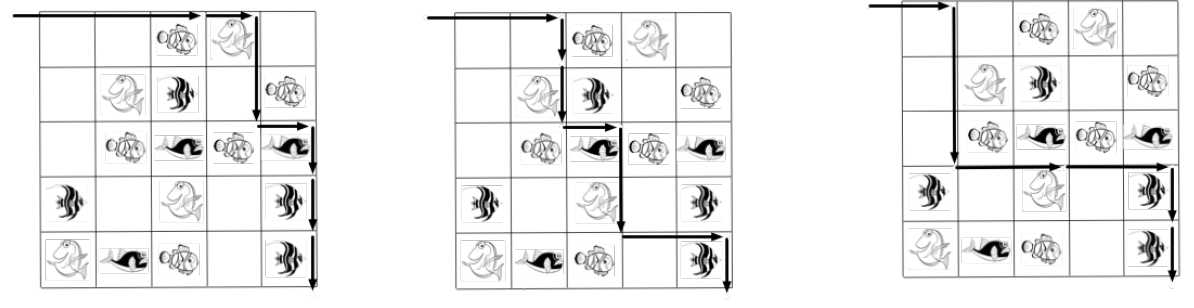
\includegraphics[width=0.75\linewidth]{lago.PNG}
    \end{figure}

    \item Sean tres cadenas de caracteres $X, Y$ y $Z$, con $|X| = n$, $|Y | = m$ y $|Z| = n + m$. Diremos que $Z$ es un \textit{shuffle} de $X$ y $Y$ si $Z$ puede ser formado por caracteres intercalados de $X$ y $Y$ manteniendo el orden de izquierda a derecha de cada cadena.

    \begin{enumerate}
        \item Muestra que \textit{cchocohilaptes} es un \textit{shuffle} de \textit{chocolate} y \textit{chips}, pero \textit{chocochilatspe} no lo es.

        \item Dise\~na un algoritmo de programaci\'on din\'amica eficiente que determine si $Z$ es un \textit{shuffle} de $X$ y $Y$. \textit{Hint}: Los valores de la matriz de programaci\'on din\'amica que construyas, podr\'ian ser valores booleanos y no num\'ericos.
    \end{enumerate}
\end{enumerate}

\end{document}
